%
\documentclass[a4paper]{article}
\usepackage[utf8]{inputenc}
\usepackage{fullpage}
\usepackage{amsmath,amssymb}
\usepackage[colorlinks,linkcolor=blue]{hyperref} % use colored text in stead of ugly boxes
\usepackage[toc]{multitoc} % Nice two-column TOC

\usepackage{graphicx}
\usepackage{tabto}
\usepackage{wrapfig}

\usepackage{pdfpages}

\usepackage{pgf}
\usepackage{tikz}

%~ \usepackage{pictures/tikz-uml}

% new line after paragraph title.
\makeatletter
\renewcommand\paragraph{\@startsection{paragraph}{4}{\z@}%
  {-3.25ex\@plus -1ex \@minus -.2ex}%
  {1.5ex \@plus .2ex}%
  {\normalfont\normalsize\bfseries}}
\makeatother

% some commands to link to files.
\newcommand{\urlRAD}{https://github.com/FelixAkk/synthbio/raw/master/deliverables/rad/rad.pdf}
\newcommand{\hrefRAD}{\href{\urlRAD}{Requirements Analysis and Design @Github}}

\newcommand{\urlTestImplementation}{https://github.com/FelixAkk/synthbio/raw/master/deliverables/test-implementation/test-implementation.pdf}
\newcommand{\hrefTestImplementation}{\href{\urlTestImplementation}{Test and Implemention plan @Github}}


\title{Programming Life - Final report}

\author{Group E:\\
Felix Akkermans \\
Niels Doekemeijer \\
Thomas van Helden \\
Albert ten Napel \\
Jan Pieter Waagmeester}

\begin{document}

\maketitle
\thispagestyle{empty}
\vfill

\small{\tableofcontents}
\pagebreak{}

\section*{Preface} ??


\pagebreak
\begin{abstract}
\noindent This document concludes the whole \textit{Contextproject} and especially the development of our product: Zelula. This piece of software provides synthetic biologists with a visual tool to design, simulate and validate biological logic circuits.

The project was roughly divided in two parts: the design stage and the implementation stage. Both were roughly of equal length.

todo fix more.
\end{abstract}
\pagebreak

\section{Introduction}
After finishing the fifth SCRUM iteration, this documents provides an overview of the product we developed, how the process went and how it compares to the plans we made in the documentation phase. 



%images used:
\pgfdeclareimage[width=0.45\textwidth]{gui-final}{pictures/gui_final1.png}
\pgfdeclareimage[width=0.45\textwidth]{gui-input-csv}{pictures/define-inputs-csv.png}
\pgfdeclareimage[width=0.45\textwidth]{gui-input-editor}{pictures/define-inputs-editor.png}
%~ \pgfdeclareimage[width=0.45\textwidth]{gui-final}{pictures/gui_final_spitscreen.png}

\newcommand{\screenshotScale}{1.4}



\section{Description of Zelula}
Zelula is a modelling and simulation package which enables users to simulate the protein \textit{logic} in a cell. With a provided set of BioBricks representing AND and NOT gates, the user is able to design interactions between the different BioBricks. The resulting circuits can be simulated, the results will be presented as a concentration/time graph.


\subsection{Circuit editor}
\begin{figure}[h!]
\centering\begin{tikzpicture}[scale=\screenshotScale]
	\pgftext[left, base]{\pgfuseimage{gui-final}}
	\draw [draw=red,very thick] (0, 2.4) -- (0, 3.7) -- (7.15, 3.7) -- (7.15,0.14) -- (1.5,0.14) -- (1.5, 2.4) -- (0,2.4);
\end{tikzpicture}
\caption{GUI mainscreen; highlighted is the workspace with the regular (draggable) gates.}
\end{figure}

\noindent Zelula enables the user to intuitively construct circuits from the basic available building blocks (see figure 1 for the mainscreen). Gates can be dragged from the sidebar to arbitrary positions in the working area. Connections between the gates can easily be dragged from and to the \textit{input} and \textit{output} connectors and the endpoints on gates. 

When a connection is made, no protein is selected for it by default. The user may select which protein to use. Visual feedback on protein assignment is provided through the colors of the connections.

The interface prevents the user to make some simple mistakes. For example, it's impossible to connect two inputs. If the user connects one output to two inputs, the interface makes sure the protein on those connections is the same.

Even the position of the circuits' input and output connectors can be freely chosen by dragging them using the text as an handle.

Removing gates and connection is a matter of double clicking on them.

\newpage
\subsection{Compound library}
\begin{figure}[h!]
\centering\begin{tikzpicture}[scale=\screenshotScale]
	\pgftext[left, base]{\pgfuseimage{gui-final}}
	\draw [draw=red,very thick] (0,0.14) rectangle (1.5, 2.5);
\end{tikzpicture}
\caption{GUI mainscreen; highlighted is the box with the (draggable) compound gates.}
\end{figure}

\noindent Every circuit can be saved as a compound gate, which means it can easily be reused in later circuits. The saved compound gates are presented to the user in the sidebar, below of the basic gates (figure 2). When a user drags a compound gate to the working area, it will expand to the original arrangement of gates, with the inner connections in place. The only thing left for the user is connecting it to the rest of its circuit.

\subsection{Validation}
When a user is satisfied with his work, he can validate the circuit. Different errors like unassigned proteins or inclomplete connections will be reported. The user will see the error message below the circuit, providing excellent overview to both the circuit and the errors to solve the problem.

\subsection{Simulation}
A valid circuit can be simulated. In order to simulate a circuit, the input must be defined as a function of time. Zelula provides two ways to accomplish this. Firstly, in an input editor the level for each input can be defined as a function of time in a visual way, secondly, a CSV text can be provided describing the transitions as a function of time.

\paragraph{Input editor}
\begin{figure}[h!]
\centering\begin{tikzpicture}[scale=\screenshotScale]
	\pgftext[left, base]{\pgfuseimage{gui-input-editor}}
\end{tikzpicture}
\caption{Dialog for defining input values per protein in client.}
\end{figure}

\noindent The input editor (figure 3) enables the user to define each input signal in a visual way. Each tick represents a number of seconds in the simulation. The user can select this number of seconds, and also the number of ticks available.

When a user clicks on a tick, it is toggled. The user may also select ranges by clicking on a certain tick an dragging the mouse to another tick while holding the mouse button.

\newpage
\paragraph{CSV input}
\begin{figure}[h!]
\centering\begin{tikzpicture}[scale=\screenshotScale]
	\pgftext[left, base]{\pgfuseimage{gui-input-csv}}
\end{tikzpicture}
\caption{Dialog for defining input values in client by CSV.}
\end{figure}

\noindent The input may also be defined by a simple CSV format (figure 4), as defined by the SA.

\subsection{Exporting}
The work done in Zelula can be shared in two different ways: the user can export the circuit to a SBML file, a common format uses in syntetic Biology.

Secondly, the visualistion of the graphs can be exported to a number of different image formats.

\subsection{Server}
The server operates in the background, serving the files needed for the GUI, providing file storage and simulation services. The user does not interact with it in a direct way.

The servlets depends on Tomcat and might be distribugted as a \verb|.war| archive. 


\section{Design and implementation process}
The first half of the project was focused on design, while the second part was all about implementation. In this chapter we will reflect on the consistency between design and implementation. We will clarify what was implemented according to the documents and what was changed or perhaps not implemented. This will done with help of a reflection on the initial GUI sketches (3.1) and our list of requirements (3.2).

\subsection{Client GUI}
In our RAD document\footnote{\hrefRAD} we gave a few simple sketches of what we had in mind for the user interface of the client. The final implementation is greatly influenced by these sketches, as can be seen from the following screenshots.\\

\begin{figure}[h!]
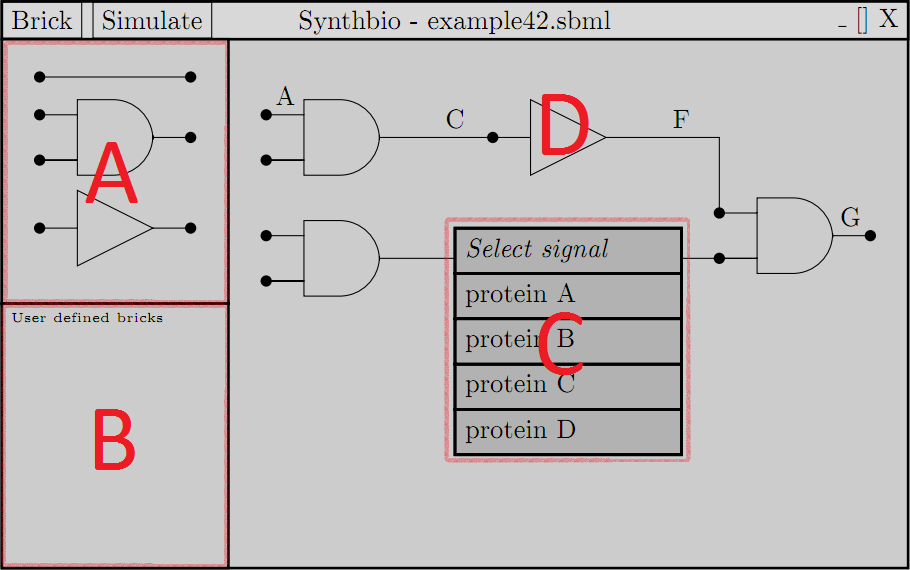
\includegraphics[width=8cm]{pictures/gui_sketch1_marks.png} 
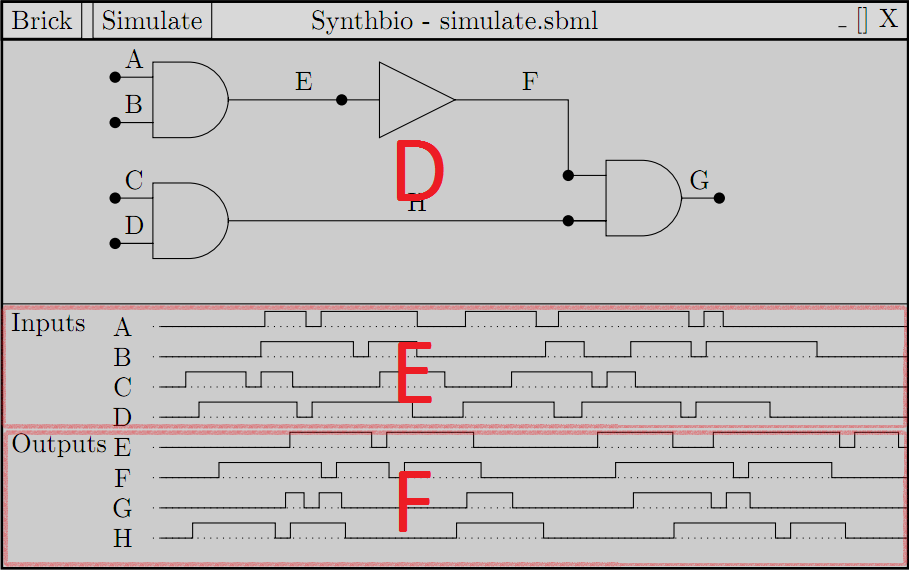
\includegraphics[width=8cm]{pictures/gui_sketch2_marks.png}
\caption{Sketches from RAD document: model and simulate.}
\end{figure}

\begin{figure}[h!]
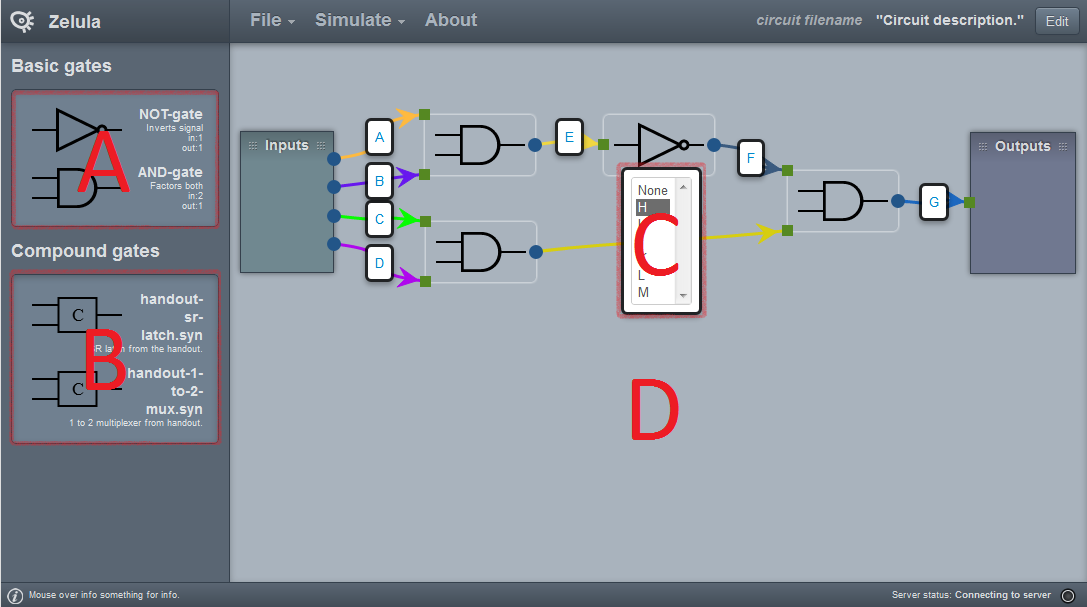
\includegraphics[width=8cm]{pictures/gui_final1_marks.png} 
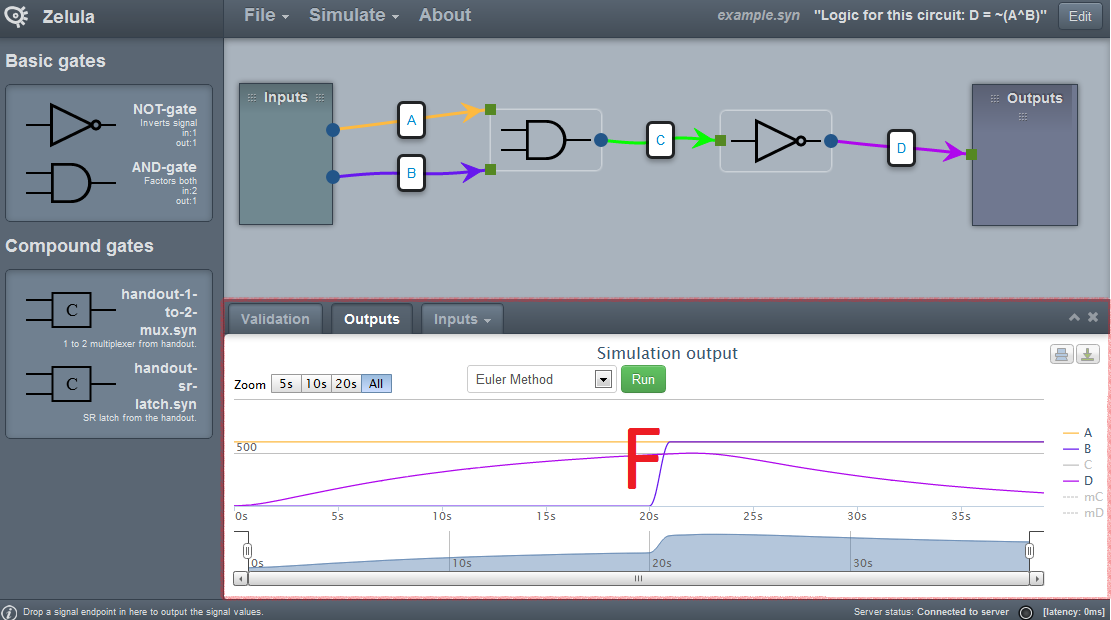
\includegraphics[width=8cm]{pictures/gui_final2_marks.png}
\caption{Screenshots of the final GUI implementation: mainscreen and outputs (F).}
\end{figure}

The matching letters in the "before" (figure 5) and "after" (figure 6) pictures show the same functionality. So A and B provide all the gates, D is the workspace, and so on. There have not been any great changes from what we had in mind for the user interface. We did, however, add a lot of features along the way; small features we did not think of at the beginning. For example, we colored the proteins so that they are easily distinctable and added general gates which serve as input or output. Another example is that used proteins cannot be chosen from during protein selection. It is according to the SCRUM-workflow that we have added these little features. We started of with a basic working product and added them along the way.

It is according to the SCRUM-workflow that we have added these little features. We started of with a basic working product and added them along the way.

Implementation was greatly accelerated by the use of frameworks and libraries such as jQuery, Bootstrap, HighCharts and jsPlumb. The use of such frameworks of course also implies the study of their use, and solving problems or limitations you encountered with them. This costed considerable time as eluded in section 4.
\newpage
\subsection{Requirements}
In the Test \& Implementation plan\footnote{\hrefTestImplementation} we set up a list of requirements according to the MoSCoW model. What follows is a copy of this list with comments on how (and if) it is implemented.

\paragraph{Must-Haves}
\begin{description}
\item[1. Connection] \textit{Client and server must be able to communicate. If there is no connection, the user should be notified.}\\
This was one of the first finished tasks, as it is essential for both client and server. The client will show an error dialog when no connection to the server can be established. While there is a connection, the user can view the connection delay (in milliseconds) in the bottom right corner of the screen.

\item[2. Available gates] \textit{The application must be able to present a list of available gates to the user. These gates can be used to model the circuit.}\\
As can be seen in figure 6.A, the user is presented with a list of draggable (regular and compound) gates.

\item[3. Design circuit] \textit{The user must be able to design a circuit by specifying gates (using a drag-and-drop) and the relations between these gates.}
	\begin{itemize}
	\item \textbf{3.1} \textit{The application must be able to visualize a gate using a simplified image. This image should relate to the function of the gate. For example, for the AND gate, it is logical to use the distinctive AND symbol normally used in circuit design.}
	\item \textbf{3.2} \textit{The user must be able to drag and drop gates from the list into the working area.}\\
	Gates are visualized using a simple, yet distinctive image (figure 6.A). They can dragged from the list and dropped into the workspace (figure 6.D).

	\item \textbf{3.3} \textit{The user must be able freely to move the gate around in the working area, but gates will snap to grid points on the working area.}\\
	After the gates are dropped into the workspace, the description of the gate disappears and the image remains. The gates can still be dragged around the screen.\\
	At first, we got the system working without a grid snapping system. This worked very well and we did not see the need to implement a grid. That is why we postponed this requirement, and decided to drop it near the end of the project.

	\item \textbf{3.4} \textit{The user must be able to draw connections between the gates in the form of wires.}\\
	In the workspace, gates get endpoints for input and output (the little green and blue dots in figure 6.D). Wires can be dragged from the output endpoints to the input endpoints. Wires from input to input and output to output endpoints are not possible. Output endpoints can contain multiple wires, while inputs only allow one.

	\item \textbf{3.5} \textit{The user must be able to draw input and output wires for the circuit, to explicitly state which proteins will be used as input.}\\
	We have added input and output gates which serve as big input or output endpoint. Wires can be dragged from the input and dropped into the output.

	\end{itemize}
\item[4. Available proteins] \textit{The application must be able to present the user with an overview of available proteins to assign to signals (visualized by the wires).}\\
Clicking Simulate $>$ Show proteins in the menu will display a table with the available proteins and matching parameters. This table is sortable and can be filtered. Each wire will also have an overlay with the selected protein. Clicking on this overlay displays a list of proteins that can still be used for selection (figure 6.D).

\item[5. Protein specification] \textit{The user must be able to specify which protein is used for a certain signal.}\\
After opening the list of unselected proteins (figure 6.D), clicking a protein results in this protein being specified for the connection.

\item[6. Export circuit] \textit{The application must to able to save a circuit to a .syn file.}\\
A circuit can be saved using File $>$ Save and exported to SBML using the File $>$ Export menu item.

\item[7. Import circuit] \textit{The application must be able to load an exported circuit from a .syn file.}\\
Saved files can be loaded using the File $>$ Open menu item.

\item[8. Input values specification] \textit{The user must be able to specify the input values used for the simulation of the circuit.}\\
Clicking Simulate $>$ Define inputs (or pressing F7) will open a dialog in which the input values can be defined (figure 6). These input values can also be loaded from a .csv file.

\item[9. Circuit validation] \textit{The user must to be able validate his circuit in the application and get feedback over where there are conflicts.}\\
Pressing F8 (or clicking Simulate $>$ Validate circuit) will give a validation of the circuit. This validation is done server side, and conflicts are grounded by useful feedback.

\item[10. Circuit simulation] \textit{The application must be able to simulate a valid circuit and present the output values to the user.}\\
Pressing F9 (or clicking Simulate $>$ Run solver) will simulate on the server and present the user with a plot of the output values (figure 6). The user can zoom in/out and specify which proteins are visible in the plot (only the input and output values are shown by default). Because we use a simulating library which supports multiple solving methods, we give the user the options to select a method.
\end{description}

\paragraph{Should-Haves}
\begin{description}
\item[11. Re-use circuits] \textit{The application can import pre-defined circuits as extra gates. This is not a necessity, but would be a great addition to the program (and will ease building circuits). Among others, protein specification, importing and exporting will be more difficult to implement.}\\
This was a requirement we really wanted to add, but decided to implement a simpler version due to time restrictions. We wanted to make it so that compound gates were visualized the same as regular gates, but decided this would be too much work. We can now mark circuits as compound gates at the time of saving. These gates will then show up in the list of compound gates and can be dragged into the workspace. When dropped, the old circuit will show up (minus the input/output signals).
\end{description}


\section{Key problems and solutions - highlights}

During this project we have encountered some problems. In this section we will have a look at some of the highlights of these problems and how we fixed them.

\paragraph{Planning and design}
Since, for some of us, this was the first time working with SCRUM, it took some getting used to. At first, we had to get used to working towards a result in two weeks and estimating what we could do. This became easier as the project progressed. 
What we really noticed is that our design was not complete. We hadn't thought of the complete structure and failed to set some standards of coding. This led to less readable code, which is annoying when reviewing each others code, and no clear idea which function was implemented where. Especially later on, some functions turned out to be double implemented or unused. This point is also discussed in the paragraph about restructuring.

\paragraph{Setup}
A common issue using server-client structure is the actual connection between the two. In the beginning we had some trouble with this but this was mainly caused by out of sync code and trouble with Apache Tomcat. We decided on a standard version of Tomcat and wrote a setup page on the wiki\footnote{\url{https://github.com/FelixAkk/synthbio/wiki/Tomcat-installation}}. Afterwards, the problem was solved.

\paragraph{QUnit}
Our program was developed test driven. This makes for very neat code, but it also comes with some problems. We mainly encountered problems with QUnit, a JQuery testing framework similar to Java's JUnit. Although the testing was done properly, the feedback on the results was not very helpful. Eventually we managed to tackle this problem with some extra manual testing. We chose to do some extra manual testing instead of switching testing framework because of all the work we already put into it. Also, QUnit works really easy with JQuery code and the code is readable. 

\paragraph{Drag and drop}
Another problem client side was the dragging and dropping of gates and connecting them with wires. We had anticipated this as being tough and found a solution in jsPlumb, a solution with its downsides. The framework jsPlumb makes it easy to create connectors and draw wires between gates, but it didn't fully meet our needs so we had to customize it, leading to quite some hours of extra work.

\paragraph{Dropdown menus}
At one point, we figured we wanted to select our proteins from dropdown menus on our wires. Regular dropdown menus from JavaScript are not an issues, however combining this with jsPlumb and bootstrap proved to be a little more difficult. This took more time than we had anticipated but was eventually solved by fully generating the menus every time we needed it. When opening a menu we just adjust its size, to simulate its dropdown effect.

\paragraph{Communication and github merging}
Throughout this project we worked with Git and GitHub to share our code. We also used the ticket mechanism of GitHub to keep track of what had to be done. Git is exceptionally good at merging code but cannot always prevent conflicts. If there is too little communication between two people who are working on the same code, merging can become difficult. However, with some reverts and recommitting these problems were resolved.

\paragraph{Restructuring}
We had a lot of code clutched together. We had that idea ourselves and the SIG evaluation gave the same result. So towards the end of our project, we did some major restructuring. We shifted some functions around, deleted unused functions, changed some names and did some more testing and commenting. On the client side we put every function into files named exactly after the part of the program they run in. This made it a lot easier to look for functions when you wanted to adjust code, or notice an error in some part of the program. 

\paragraph{Solver issues}
During the second to last iteration we discovered a problem with the connection to the solver which was implemented. It didn't show correct results for the transcription and translation reactions, because degradation didn't work. After discussing things with Alexey, Jan Pieter decided to write a solver on its own, which initially took about 12 hours of work. Cleaning up the code and some other adjustments took another 8 hours.
During the development of our own solver, Albert worked together with Alexey to fix the problems in the first approach. The result of this is the availability of two solvers in our GUI.

\paragraph{Graph rasterisation, servlet issues}
The graph library used in our GUI provides a way to export the graph to different image formats. This exporting requires a special server which is provided by the author of the library, but we wanted to be independent of that, so we decided to provide the rasterisation service by our own server code.
At first, it seemed very straight-forward, but quite some time was absorbed by the confusion about Tomcat's class-path. It turns out Tomcat only looks in \verb|WEB-INF/lib/*| and not in it's subdirectories, resulting in a huge stack of \verb|NoClassDefFoundErrors| to fix.

In the second to last iteration we discovered that our simulator didn't degrade anything (Figure~\ref{fig:wrong}), this was discovered so late because non of the tests targeted degradation, we only tested if the reaction speed changed. Either the solver library (SBMLsimulator) was wrong or the SBML format used was. After some testing and help from Alexey, the problem found was indeed the SBML format.\\

\begin{figure}[h!]
	\centering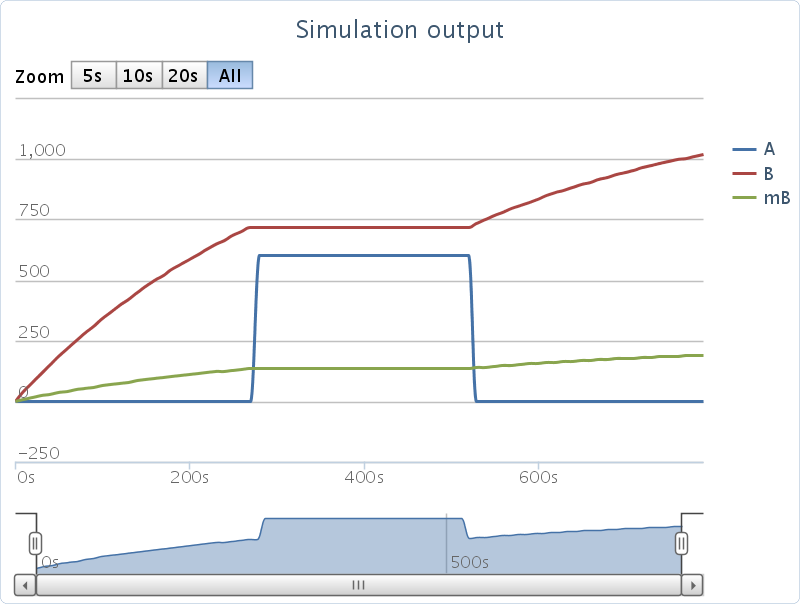
\includegraphics[scale=0.35]{../../screenshots/2012-05-31-not-output.png}
	\caption{Wrong output, B doesn't degrade.}
	\label{fig:wrong}
\end{figure}

\noindent The SBML format that is used for the simulation requires a list of species and a list of reactions. These reactions each have a set of reactants, products and modifiers:
\begin{itemize}
	\item reactants are the fuel of the reactions, the reactants decrease as the reaction occurs,
	\item products are what the reaction produces in the end, the products increase as the reaction occurs,
	\item modifiers can speed up or slow down the reaction, but their concentration doesn't change in the reaction.
\end{itemize}
In our simulation we have two reactions: transcription and translation. The transcription reaction produces mRNA (that encodes for a specific protein) from a gene sequence with help from transcription factors. The translation reaction produces the protein from the mRNA. On top of this degradation takes place: the proteins and mRNA degrade over time.\\
\\
In our SBML file the degradation didn't have a separate reaction, which caused a problem given that the degradation reaction required a different set of reactants, products and modifiers from the transcription and translation reactions.\\
The transcription reaction produces something from a gene sequence. The degradation reactions need to degrade to something, but it's not producing something from a gene sequence, so putting the degradation in the same reaction as the transcription (or translation) reaction would be wrong since they have different reactants and different products.\\

\begin{wrapfigure}{l}{8cm}
	\centering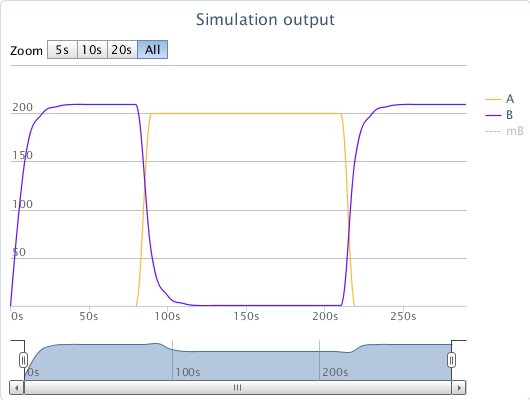
\includegraphics[scale=0.5]{../../screenshots/2012-06-14-not-output.png}
	\caption{Correct output, B degrades.}
	\label{fig:correct}
\end{wrapfigure}

To fix this (Figure~\ref{fig:correct}) we split the transcription and translation reactions such that the degradations got their own reactions, this allowed us to specify different reactants, products and modifiers for the degradation.


\section{Reflection on the teamwork}

\section{Individual reflection on the project} %max 1 A4 per teammember
\subsection{Felix Akkermans}
\subsection{Niels Doekemeijer}
Looking back at this project, I am quite pleased with the overall teamwork and final result. I feel like we had a bit of a rough start, having very few meetings in the first part of the project. This resulted in somewhat lower grades than expected for the first few documents. Writing reports is not my favourite part of projects, but it has to be done and I did my share.

After starting implementation of the product, I feel like the group came more at ease (having more weekly meetings definitely helped, too). I had never worked with SCRUM before, but I can see why it's accepted as a development method as it definitely helps to always have a working product. Demonstrations after each iteration helped us confirm that we were well on our way. We put a lot more work in the implementation than in the reports, but I think both were of very decent level.

I started taking more initiative in the implementation phase and tried to always have an overview over what was happening and what needed to be done. My opinion is that every group member had a phase in which they did a lot of work and a phase in which they did less than usual. I think the overall activity and devotion to the project was good. This has lead to a decent product which has exceeded my initial expectations.

This high activity and devotion sometimes lead to "code-clashes" as more people accidentally worked on the same bit of code. I personally think these little conflicts are no big deal and I rather have work being done twice than work not being done at all. It did not affect our team work and I think we settled these few miscommunications well.

\subsection{Thomas van Helden}
I am quite amazed about the product we managed to put together. I'm certainly glad we made it with a nice JS GUI. Previous projects were all made in Java leading to horrific GUIs. This project is also the most complex product I've ever made. So in several ways, this was the most challenging IT project I've worked on. Once again, I've learned that a good preparation works a million times better than just starting to code. 

My reflection on the teamwork can be divided into three parts: A general part, feedback on my work and communication about the product.
In general I was very pleased with the team. We all started every sprint with a meeting. We discussed the issues in the previous sprint and we divided the work. Although some did more than other, we all had an understanding mindset towards each other.

I believe the biggest part was the feedback on me. I personally feel as if I really didn't do the job I could normally do. I was occupied with a lot of things, personal and professional, and so I was unable to do my job properly. This was discussed in the team and I got some really good feedback on how to improve my attitude towards the team. 

Communication, in what I've learned so far, is always an issue. Although we did a good job, there was still some miscommunication leading to extra work and stress. It happened a few times that people were working on the same thing without the other one knowing. This resulted in two people doing double work, wasting hours of time. This was no real disaster but it was a shame. Apart from these few points there was nothing to mention with regard to our teamwork.

\subsection{Albert ten Napel}
I think the project has been very successful, the resulting product is a beautiful, easy to use application that has quite a few useful functions. The teamwork itself was pretty good, we had a meeting each scrum iteration planning on what we would do that iteration. This way I knew what I should do and what was expected of me. In previous projects I was often not sure on what I was to do and the planning was really weak. We also used GitHub, which allowed us to create issues detailing things like optional tasks, bugs and unassigned work. When I was finished with a task and I didn't have anything to do, I could check the issues and pick a new task.\\
\\
Communication was mostly good, if somebody had a problem he could tell it to the group and we would all think about it. There was some miscommunication regarding tasks that two people were doing at the same time without the other knowing. But in the end this was solved fairly quickly and wasn't that big of a problem.\\
\\
During the project I learn to better manage things, for example using tools like ant. I also learned how to set up a server-side system with Tomcat and Java Servlets and how to manage libraries in Java. Furthermore we used git instead of svn (which was used in earlier projects), I learned a lot about how to use git.\\
Test driven design wasn't something that I liked a lot. In theory I like the idea but in practice I find writing all of the tests upfront more of a burden and a lot of time was spent actually fixing tests instead of fixing code.\\
\\
I didn't do a lot of client side, JavaScript things, because early on I wasn't very interested in that part of the application. Later on I didn't feel confident that I could help with the JavaScript stuff because I wasn't very familiar with the client side. I think I should have done a bit more, since I would've learned some things and with a next project I would like to look more into the GUI side of things.

\subsection{Jan Pieter Waagmeester}
The first thing I would like to note is that I am surprised by the final product we managed to deliver, it exceeds my expectation. I looks good, works well, has clean code and all the must-haves we defined. Overall, I am also satisfied with the way the team worked together. There were some frustrations now and then, but always room for feedback. 

I will reflect in more detail on two areas: the technical development and the team collaboration.

\paragraph{Development \& tool use}
% Development process, TDD, tool use.
It was quite some time ago since I did collaborative Java development on larger scale. So I did not have strong opinions about the tool chain to be used, however, during the Software testing class I got my share of Eclipse frustration, so glad to leave that for a while.

I'm used to the command line and enjoyed learning to use new tools like \verb|tomcat|, \verb|ant|, \verb|git|. Tomcat is a very complicated way to have simple server functionality. Since we only needed exactly that, it might have been more efficient to select something more lightweight, however, lots of documentation is available. Ant is a powerful way of to automate boring tasks and made me smile from time to time. Git, especially in combination with GitHub beats every other SCM toolchain I have used before. Easy of branching makes it useful, local commits make code review by peers way easier, but like any other SCM depends on how it's used.

The actual development was often quite straightforward. No very complicated algorithms, mostly pushing simple data structures around. That said, testing things is not always easy. For example, testing JSON responses is not a trivial task if the testing tools have no notion about its structure. I think we could have put more focus on exactly what to test, not only on line or branch coverage.

I really did like the test driven design approach. Some refactoring made the importance of tests very clear: the tested parts worked like before because problems were identified by the tests, but the untested functionality lagged behind.


\paragraph{Team collaboration}
% balance of work, Initiative. SCM frustration
Balancing the work during projects is an always an issue. Some people have less time available, some like to invest more time. Some are perfectionists, others do not care about brace placement. I think being one of the more active people does not always justify complaints about others contributing less. Some people could have displayed more initiative from time to time.

Working together in a source code management system can be a source of frustrations: braking \textit{the make}, little care when committing unintentional changes or merges. I sometimes found it hard to patiently correct them and explain the how and why.


\section{Lightweight SCRUM Plans}
The following pages will include the relevant parts of our lightweight scrumplans for each iteration. The colored links and numbers with a hashtag refer to GitHub issues on \url{https://github.com/FelixAkk/synthbio/issues}. For each iteration, a milestone is available providing a nice overview of the issues for each iteration.

\includepdf[
	landscape, frame, nup=1x2, pages=2-3,
	addtotoc={2 , subsection , 1 , Scrumplan 1 , scrum-1}
]{../scrumplan-1/scrumplan-1.pdf}

\includepdf[
	landscape, frame, nup=1x2, pages=2-3,
	addtotoc={2 , subsection , 1 , Scrumplan 2 , scrum-2}
]{../scrumplan-2/scrumplan-2.pdf}

\includepdf[
	landscape, frame, nup=1x2, pages=2-3,
	addtotoc={2 , subsection , 1 , Scrumplan 3 , scrum-3}
]{../scrumplan-3/scrumplan-3.pdf}

\includepdf[
	landscape, frame, nup=1x2, pages=2-3,
	addtotoc={2 , subsection , 1 , Scrumplan 4 , scrum-4}
]{../scrumplan-4/scrumplan-4.pdf}

\includepdf[
	landscape, frame, nup=1x2, pages=2-3,
	addtotoc={2 , subsection , 1 , Scrumplan 5 , scrum-5}
]{../scrumplan-5/scrumplan-5.pdf}


\end{document}